\documentclass{article}
\usepackage{graphicx}
\usepackage{multicol} % use to multiple column in itemize
\usepackage{float}
\usepackage{setspace}
\usepackage{hyperref}
\setlength{\parskip}{0.5em}

\begin{document}

\title{Classification}
% \author{Cong Cuong PHAM}

\maketitle

\begin{abstract}
This document introduces some fundamental notions of Classification.
\end{abstract}

\subsection{Classification (Supervised)}
\par The goal of classification is to find what class a sample belongs to.

A class could be something like Windows 10 Mobile, and a sample could be something like phone. To get classification working, you have to feed the machine learning algorithm a decent amount phone examples, some of them labeled Windows 10 Mobile, and others labeled, well... non-Windows 10 Mobile. With enough training samples, a classifier will eventually be able to generalize what similarities constitute a Windows 10 Mobile phone and voilà, you've trained a computer to figure out phone types!

\begin{figure}[H]
\centering
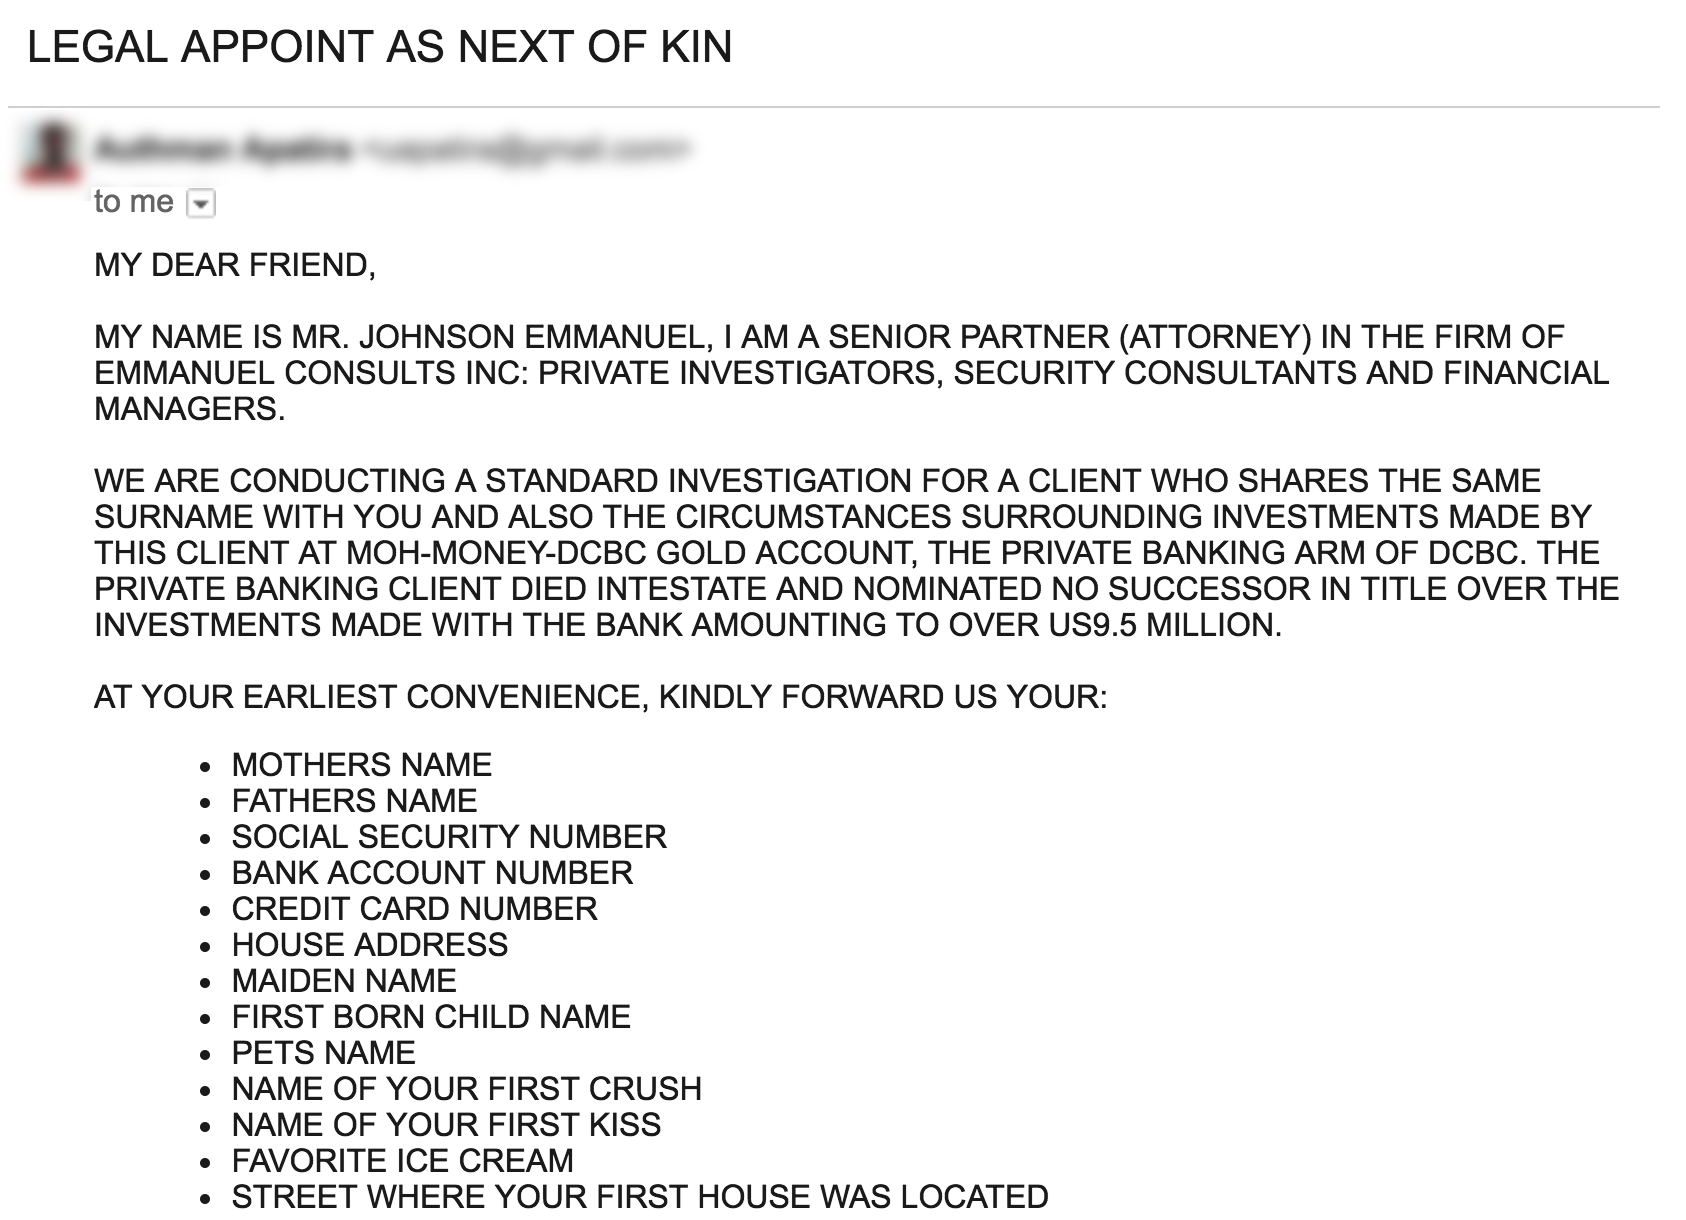
\includegraphics[width=0.8\linewidth]{pic/classification.png}
\caption{Example of classification.}
\end{figure}

More examples

\begin{itemize}
    \item Given a list of emails marked spam and not-spam, figure out if a newly received message is actually spam or not.
    \item Given many images of your friends, perform facial recognition on a brand-new, never-before seen image of one of your friends.
    \item After being trained with a few books, decide which of the before seen authors wrote an article.
    \item Given a list of physical symptoms, determine what ailment a person has.
\end{itemize}

\par Classification falls into the realm of supervised learning because in order for it to work, you have to guide the computer by proving it with examples of correctly labeled records. Once you're done training the computer, you can test it by seeing how accurately it scores those records.

\begin{flushright}
    source: \href{https://courses.edx.org/courses/course-v1:Microsoft+DAT210x+6T2016/courseware/e36e6b45ae5d4032bef2ec557c1ff48f/a8cf8333f6044e9b9a357b7797f282e3/?child=first}{course.edx.org}  
\end{flushright}
\end{document}